\documentclass[tikz,border=4pt]{standalone}
\usepackage{amsmath,amssymb}

\usetikzlibrary{arrows.meta,positioning,automata,shapes,shapes.misc,calc,decorations.pathmorphing,decorations.markings,angles,quotes,patterns,mindmap,matrix,knots,hobby,trees}
\tikzset{->-/.style={decoration={markings, mark=at position 0.5 with {\arrow{Stealth}}}, postaction={decorate}}}
\begin{document}
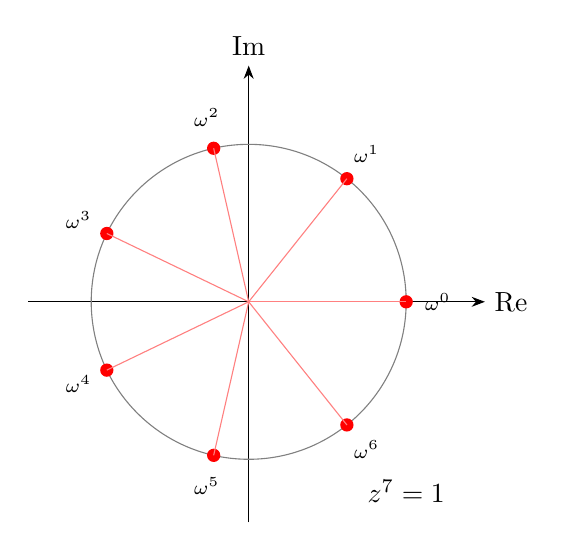
\begin{tikzpicture}[scale=2, >=Stealth]
\draw[->] (-1.4,0) -- (1.5,0) node[right] {$\mathrm{Re}$}; \draw[->] (0,-1.4) -- (0,1.5) node[above] {$\mathrm{Im}$};
\draw[gray] (0,0) circle (1);
\foreach \k in {0,...,6} { \fill[red] ({360/7*\k}:1) circle (1.2pt); \draw[red!50, thin] (0,0) -- ({360/7*\k}:1); \node[font=\scriptsize] at ({360/7*\k}:1.2) {$\omega^{\k}$}; }
\node at (1,-1.2) {$z^7 = 1$};
\end{tikzpicture}
\end{document}
